\documentclass[11pt]{article}
\usepackage[T1]{fontenc}
\usepackage[margin=1in]{geometry}
\usepackage{amsmath,amssymb,amsthm}
\usepackage{mathtools}
\usepackage{enumitem}
\usepackage{setspace,microtype}
\usepackage[pdfusetitle,bookmarksnumbered]{hyperref}
\newcommand{\la}{\langle}
\newcommand{\ra}{\rangle}
\newcommand{\N}{\mathbf{N}}
\newcommand{\Z}{\mathbf{Z}}
\newcommand{\Q}{\mathbf{Q}}
\newcommand{\R}{\mathbf{R}}
\newcommand{\where}{\,|\,}
\newcommand{\abs}[1]{\lvert #1 \rvert}

\usepackage{graphicx}
\graphicspath{ {image/} }

\usepackage{mathpazo}
\usepackage[scaled=1.008]{inconsolata}
\usepackage[scaled=0.842]{berasans}

\makeatletter
\let\@subtitle\@empty % default value
\protected\def\subtitle#1{\gdef\@subtitle{#1}}
\def\@maketitle{%
  \newpage
  \begin{center}%
  \let \footnote \thanks
    {\Large \@title \par}%
    {\@subtitle \par}%
    \vskip 0.5em%
    {\lineskip .5em%
      \begin{tabular}[t]{c}%
        \@author
      \end{tabular}\par}%
    {\@date}%
    \vskip -0.5em%
  \end{center}%
  \par}
\makeatother

\title{Notes on Elementary Stochastic Processes}
\author{Cheng, Feng}
\subtitle{based on MAT 135B}
\date{}

\onehalfspacing
\setlength{\parskip}{0.25em}
\setlist{listparindent=\parindent,parsep=0pt}

\begin{document}
\maketitle

% ------------------------------------------------------------
% MadHat notebook page 1: DTMC
% ------------------------------------------------------------

\setcounter{secnumdepth}{0}

\section{Discrete Markov Chains}

\subsection{Introduction}
Definition.
\[
P(X_{n+1}=i_{n+1} \where X_{n}=i_{n},X_{n- 1}=i_{n- 1},\dots ,X_{0}=i_{0})=P(X_{n+1}=i_{n+1} \where X_{0}=i_{0})
\]
(We are only considering homogeneous Markov chains here, whose one-step transitional probabilities are unrelated to the values of $n$.)

Three elements: the state space $S$, the transitional probabilities represented by the stochastic matrix $P$, and the initial distribution $\alpha $.

The stochastic matrix $P$ is given by the transitional probabilities $p_{ij}$ from state $i$ to state $j$ ($i,j\in S$) in a single step. It is obvious that the row sums of $P$ is equal to 1.

There is a one-to-one correspondence between a Markov chain with initial distribution $\alpha $ and transitional stochastic matrix $P$ and a sequence $\{X_{n}\}_{n\geq 0}$ satisfying
\[
P(X_{0}=i_{0},\dots ,X_{n}=i_{n})=\alpha _{i_{0}}p_{i_{0}i_{1}}\dots p_{i_{n- 1}in}
\]
We also have the extended Markov property and the strong Markov property. Both are very useful tools in the theory of Markov chains.
The former states that the future event $F$ depends solely on the current state $\{X_{n}=i\}$, regardless of the past history $H$.
The latter says that under finite stopping time $T$ (such that the event $\{T=n\}$ is determined solely in terms of $X_{0},X_{1},\dots ,X_{n}$), the sequence of events $\mathbf{X' }$ starting from time $T$ is a new Markov chain with the same transitional probabilities and is unrelated to the history before $T$.

The fact that $n$-step transition probabilities can simply be represented by the $n$-th power of the transition matrix $P$ is due to the Chapman-Kolmogorov equations:
\[
p_{ij}^{m+n}=\sum_{k\in S}p_{ik}^{m}p_{kj}^{n},
\]
which break down the calculation of $n$-step transition probabilities.

It is customary to use a row vector to represent the initial distribution $\alpha $. We may then calculate the distribution at time $n$ directly by $\alpha P^{n}$, a row vector as well.

\subsection{Classification of States}
We say $j$ is \textit{accessible} from $i$ (denoted by $i\rightarrow j$) if $p_{ij}^{n}>0$ for some $n\geq 0$, i.e., state $j$ can be visited from state $i$ in a finite number of steps. $i \leftrightarrow j$ means state $i$ and state $j$ are mutually accessible, that the two states \textit{communicate}.

It is not hard to show that $\leftrightarrow$ is an equivalence relation, which implies a Markov chain can be reduced to \textit{communicating classes}, all of which contain states that communicate with one another. These individual classes have many useful properties. An \textit{irreducible} Markov chain has itself as the only communicating class.

Here we introduce the notion of recurrence and transience. A state $i$ is \textit{recurrent} if it is certain that $i$ will return to $i$ after a finite number of steps. A state is \textit{transient} if it is not recurrent.

If we define the first-passage time of state $i$ as
\[
T_{i}=\inf \{n\geq 1:X_{n}=i\},
\]
then the state $i$ is recurrent if $P(T_{i}<\infty )=1$, and it is transient if $P(T_{i}=\infty )>0$. (Note that if the set $\{n\geq 1:X_{n}=i\}$ is empty, then we let $T_{i}=\infty $. Random variables similar to $T_{i}$ in stochastic processes are customarily defined to also include $\infty $.)

Alternatively, if we simply define $f_{i}$ to be the return probability of state $i$, $f_{i}=1$ means $i$ is recurrent, and $f_{i}<1$ means $i$ is transient.

Writing the expectation of $V_{i}$, the number of returns to $i$, in terms of indicators with respect to $\{V_{i}\geq k\}$ (by the strong Markov property) and $\{X_{n}=i\}$, we can show that
\[
\sum_{n=1}^{\infty }p_{ii}^{n}=\infty 
\]
if $i$ is recurrent, and
\[
\sum_{n=1}^{\infty }p_{ii}^{n}<\infty 
\]
if $i$ is transient.

\noindent \fbox{\textit{Remark.}} $V_{i}+1$ here actually follows Geometric$(1- f_{i})$ for $f_{i}\neq 1$. Furthermore, we can use $P(V_{i}\geq k)=f_{i}^{k}$ for any $k\in \Z^+$ (which we get from the calculation above) to show that $P(V_{i}=\infty )=1$ for any recurrent $i$, and $P(V_{i}<\infty )=1$ for any transient $i$.

In summary, recurrence/transience can be characterized in terms of the first-passage time $T_{i}$, the sum of transition probabilities $\sum_{n}p_{ii}^{n}$, or the number of returns 
\[
V_{i}=\abs{\{n\geq 1:X_{n}=i\}}.
\]
It should be noted that finite first-passage time $T_{i}$ does not imply $E(T_{i})$ is finite as well, though the contrary is true by Markov’s inequality. This tells us we need a stronger kind of recurrence. The \textit{mean recurrence time} is the expected first-passage time
\[
m_{i}=E(T_{i})=\sum_{n=1}^{\infty }nP(T_{i}=n).
\]
When $i$ is transient, namely $P(T_{i}=\infty )>0$, $E(T_{i})$ diverges to $\infty $. On the other hand, when $i$ is recurrent, namely $P(T_{i}<\infty )=1$, if $E(T_{i})<\infty $, $i$ is \textit{positive recurrent}, while if $E(T_{i})=\infty $, $i$ is \textit{null recurrent}.

As it turns out, both recurrence and positive recurrence are class properties, i.e., all states in a communicating class should be simultaneously (not) recurrent and simultaneously (not) positive recurrent. To show recurrence/transience as a class property, one uses the Chapman-Kolmogorov equations and $\sum_{n}p_{ii}^{n}=\infty $ and $<\infty $. The most direct way of showing positive recurrence as a class property involves invariant distribution, which we will mention later.

The \textit{period} $d_{i}$ of a state $i$ is given by the gcd of all possible steps needed to return to $i$. Formally, we write $d_{i}=\gcd\{n:p_{ii}^{n}>0\}$. The state $i$ is \textit{aperiodic} if $d_{i}=1$, and is \textit{periodic} if $d_{i}>1$. Using the Chapman-Kolmogorov equations, it is not hard to show that period is also a class property.

Here we provide a summary of some elementary facts useful in judging the properties of states and classes in a Markov chain:

A subset $S_{0}$ of the state space $S$ is \textit{closed} if $p_{ij}=0$ for any $i\in S$ and state $j$ not in $S$. Using ordinary language, this means $S_{0}$ can only be accessible within itself.

\begin{itemize}

\item Consider a closed subset $S_{0}$ with finitely many states. Starting from an arbitrary state in $S_{0}$, we can write all the visits into a sequence of random variables. There must exist a state that is visited an infinite number of times. This implies every such $S_{0}$ has at least one recurrent state.

\item If we know some state $j$ is accessible from a recurrent state $i$, in reverse $i$ will also be accessible from $j$ because the probability of never visiting $j$ from $i$ ($p_{ij}^{\infty }$) is 0. Thus, the two states communicate. It follows that the set of all states accessible from any recurrent state $i$ of a Markov chain forms its recurrent class that we have discussed above.

\item Therefore, any recurrent class $C$ is a closed subset of states since any state in $C$ cannot have access to, or communicate with, any state outside $C$. In particular, in reverse, if a communicating class is closed and \textbf{finite-state}, then it contains a recurrent state. Thus, this class is recurrent. (If the class has infinitely many states, then this does not necessarily hold. The asymmetric random walk on $\Z$ has $\Z$ as the only class, which is actually transient.)

\end{itemize}

Thus, in a finite-state communicating class, there is an iff relationship between the class being recurrent and the class being closed. In the general context of finite-state Markov chains, we may now determine recurrence/transience solely based on whether the class is closed or not. This is indeed very useful.

Note that all these facts concerning a single class or a closed subset of states could be directly applied to irreducible Markov chains, quite obviously.

\subsection{Limiting Probabilities and Invariant Distribution}
Many of the theorems that occur in this section assumes irreducibility and positive recurrence of the chain. Before looking at the theorems (ideas of which are simple but the proofs are complicated), remember that a finite irreducible Markov chain is necessarily positive recurrent (we skip the proof). This is oftentimes the problem setting we will encounter.

First, we define the \textit{invariant distribution} (or \textit{stationary distribution}). The invariant distribution is invariant under the passage of time; formally speaking, if we take the convention of writing distributions into a row vector $\pi $ over the state space $S$ with sum 1, the invariant distribution needs to satisfy $\pi P=\pi $. ($\pi $ here is the left row eigenvector for eigenvalue $1$ of $P$.)

The upcoming theorems all focus on irreducible Markov chains. Now we introduce the fundamental theorem (the proof of which is completely skipped because of its technicality). In an irreducible chain, an invariant distribution $\pi $ exists iff all states are positive recurrent iff we know some state is positive recurrent, and the $\pi $ is \textbf{uniquely} given by
\[
\pi _{i}=\frac{1}{m_{i}},
\]
the reciprocal of the mean recurrence time of state $i$. This tells us that the invariant probability times the mean recurrence time at state $i$ should be 1. Also, irreducible Markov chains allow either none or only one invariant distribution.

This implies that as long as we have found one invariant distribution $\pi$ [by the Markov chain being symmetric or doubly stochastic (which we will cover soon) over all states, e.g., without referring to $m_{i}$ or even the formula $\pi P=\pi $], it is the only invariant distribution desired.

It follows from our intuition that the invariant probability $\pi _{i}$ might as well be interpreted as the proportion of time spent at this state $i$. It turns out that this is true in the limit; we can prove formally via the weak law of large numbers that under the same assumption of irreducibility and positive recurrence,
\[
\frac{V_{i}(n)}{n} \overset{P}{\to} \frac{1}{m_{i}}=\pi_i \quad \text{as} \quad n \rightarrow \infty ,\]
where $V_{i}(n)$ represents the number of times state $i$ is visited before time $n$, regardless of the initial distribution of $X_{0}$.

If we add the further condition of aperiodicity, then for any $i,j\in S$,
\[
\lim _{n\rightarrow \infty }p_{ij}^{n}=\pi_{j}.
\]
This is the so-called convergence to equilibrium theorem, which implies that the transition probability from any \textbf{arbitrary} state $i$ to a fixed $j$, in the long run, will become the invariant distribution of the state $j$. The proof of this strong theorem requires the \textit{coupling} technique.
(Note in particular that the previous theorem is concerned with the convergence of the random variable $\frac{V_{i}(n)}{n}$ in probability, while this theorem is the convergence of a sequence of numbers $p_{ij}^{n}$.)

If we extend this theorem to Markov chains in general with period $d$, we need to modify our conclusion as follows: for any $i,j\in S$, there exists a particular remainder 
$0\leq r\leq d- 1$ such that
\[
\lim _{m\rightarrow \infty }p_{ij}^{md+r}=d\pi _{j}=\frac{d}{m_{j}}.
\]
In addition, for the $n$’s that are not congruent to $r$ modulo $d$, $p_{ij}^{n}=0$. The reason behind this is that $i$ can only reach $j$ in congruent numbers of steps modulo $d$. The vague intuition behind this formula is that since $j$ may only be visited once in $d$ steps, the probability of visiting state $j$ among every $d$ steps is given $d$ times the “weight” of $j$,
\[
\pi _{j}=\frac{1}{m_{j}}.
\]
The actual proof of this is quite involved.

Another point we want to address here is the invariant distribution for a doubly stochastic Markov chain. A Markov chain is \textit{doubly stochastic} if each column sum of the transition matrix is also 1, i.e., for all $j\in S$, $\sum_{i\in S}p_{ij}=1$.

As a matter of fact, if an irreducible Markov chain is doubly stochastic over a finite state space $S$, it follows that the unique invariant distribution is uniform over all states:
\[
\pi =\frac{1}{\abs{S}}
\begin{bmatrix}
    1 & \cdots & 1
\end{bmatrix}.
\]
To show this, note that $ \begin{bmatrix}
    1 & \cdots & 1
\end{bmatrix} P = \begin{bmatrix}
    1 & \cdots & 1
\end{bmatrix}$ because the column sums of $P$ are all 1. We then just have to “normalize” the row vector to row sum 1.

Informally speaking, a Markov chain is reversible if the sequence of random variables 
$X_{0},X_{1},\dots $ running under the invariant distribution $\pi $, when looking backward from any time $t$, is what might occur in the original forward chain with the same probability. To describe this formally, the new sequence of random variables $\mathbf{Y}$ should share the same p.m.f.\ with the original chain $\mathbf{X}$:
\[
\{Y_{0}\coloneqq X_{t}=i_{0},Y_{1}\coloneqq X_{t- 1}=i_{1},\dots ,Y_{t}\coloneqq X_{0}=i_{t}\} \overset{D}{=} \{X_{0}=i_{0},X_{1}=i_{1},\dots ,X_{t}=i_{t}\}.
\]
As a result, we cannot tell whether the reversible chain is running forward or backward by looking at the sequence of $t$ random variables.

If the forward chain has its invariant distribution $\pi $ as the initial distribution, it is not hard to show that the backward sequence $Y_{0},Y_{1},\dots ,Y_{t}$ is a Markov chain with initial distribution $\pi $ as well, and with backward transition probabilities given by
\[
P(Y_{m+1}=X_{k}=i \where Y_{m}=X_{k+1}=j)=\frac{\pi _{i}p_{ij}}{\pi_{j}}.
\]
The fact that the backward sequence is also Markov rephrases reversibility to saying that the forward and backward chains share the same transition probabilities. Here comes the actual definition:

Let $\mathbf{X}$ be an \textbf{irreducible} Markov chain with $X_{0}$ having the invariant distribution $\pi $. If its time-reversal $\mathbf{Y}$ has the same transition matrix $P$ as $\mathbf{X}$ does, or simply \[
\pi _{i}p_{ij}=\pi _{j}p_{ji} \text{ for all } i,j\in S,\]
then we call $\mathbf{X}$ \textit{reversible}. (The equations above are known as the \textit{detailed balance equations}.)

\noindent \fbox{\textit{Remark.}} Reversibility is by assumption restricted to irreducible positive recurrent Markov chains. This is because we only want to determine the reversibility of a chain based on \textit{only} one invariant distribution. Also, the detailed balance equations allows only one solution.

Next, we show that in an irreducible chain, if a distribution $\lambda$ satisfies the detailed balance equations $\lambda _{i}p_{ij}=\lambda _{j}p_{ji}$, then $\lambda $ is the unique invariant distribution:
\[
\sum_{i\in S}\lambda _{i}p_{ij}=\sum_{i\in S}\lambda _{j}p_{ji}=\lambda _{j}\sum_{i\in S}p_{ji}=\lambda _{j} \implies \lambda P=\lambda .
\]
This property gives us an easy criterion for finding the invariant distribution. A direct application of this appears in the \textit{random walk on weighted graphs}. Given the probability from $i$ to $j$
\[
p_{ij}=\frac{w_{ij}}{\sum_{k}w_{ik}}
\]
based on the proportion of weight, let
\[
\lambda _{i}=\frac{\sum_{k}w_{ik}}{\sum_{i,k}w_{ik}}
\]
be the proportion of the the weight out from $i\in S$ over the total weight. We now have
\[
\lambda _{i}p_{ij}=\frac{w_{ij}}{\sum_{i,k}w_{ik}}=\lambda _{j}p_{ji}.
\]
When the weighted graph is connected, it is irreducible and thus $\lambda $ is our desired invariant distribution of the chain. The weighted graph can have self-edges because $p_{ii}$ does not affect the detailed balance equations.

If we simply take all the edge weights to be 1, it follows that $\pi _{i}=\frac{\deg(v_{i})}{2 \abs{E}}$.



% ------------------------------------------------------------
% MadHat notebook page 2: Branching Processes
% ------------------------------------------------------------

\newpage
\section{Branching Processes}

The branching process is a stochastic process that emulates the spread of a family name. There is only a single individual at time 0, represented by $X_{0}=1$. Every individual $W_{j}$ in any generation has an i.i.d.\ \textit{offspring distribution}, given by the p.m.f.
\[
p_{i}\coloneqq P(\text{number of offspring}=i),i=0,1,2,\dots .
\]
The offspring from the individual $W$ will appear in the next generation. The trivial case 
$p_{i}=1$ for some $i$ is mostly ignored.

It should be noted that a branching process is discrete and non-negative integer-valued. This suggests that we should use the method of probability generating function to investigate the properties of branching processes. Every $W_{j}$ in generation $n- 1$ is i.i.d.\ with p.g.f.\ $G(s)$, and thus we may apply the p.g.f.\ random sum formula to get
\[
G_{n}(s)=G_{n-1}(G(s)),
\]
where the subscript tells the generation the p.g.f.\ is about. Since $G_{0}(s)=s$, $G_{n}$ becomes the $n$-th iterate of $G$ for all non-negative integers $n$.

It follows that $E(X_{n})=G_{n}'(1)=G_{n- 1}'(G(1))G'(1)=G_{n- 1}'(1)E(W)=E(X_{n- 1})\mu $, which gives us the formula $E(X_{n})=\mu ^{n}$, if we denote $E(W)$ by $\mu $.

This indicates that when $\mu <1$, $E(X_{n})\rightarrow 0$; when $\mu =1$, $E(X_{n})\rightarrow 1$; and when $\mu >1$; $E(X_{n})\rightarrow \infty $ as $n\rightarrow \infty $.

Define $e_{n}=P(\{X_{n}=0\})$, the extinction probability at $n$-th generation. Since $\{X_{n}=0\}$ is an increasing sequence of events, the ultimate extinction probability
\[
e=P(\cup _{n=1}^{\infty }\{X_{n}=0\})=\lim _{n \to \infty }e_{n}.
\]
This extinction probability $e$ is actually the smallest non-negative solution to $G(x)=x$. To prove this, first note $G_{n}(0)=P(X_{n}=0)=e_{n}$ and recall $G_{n}(s)=G(G_{n- 1}(s))$ because $G_{n}(s)$ is the $n$-th iterate of $G$. Thus,
\[
e_{n}=G(e_{n- 1}) \text{ for all } n\in \N .
\]
Take $n\rightarrow \infty $ on both sides, we have $e=\lim _{n\rightarrow \infty }G(e_{n})$. $G(x)$ is uniformly convergent on 
$[0,1]$ and is thus continuous on $[0,1]$. Therefore, since all $e_{n}\in [0,1]$, by the preservation of sequential limit under continuity, $e=\lim _{n\rightarrow \infty }G(e_{n})=G(e)$.

Beyond the fact that $e$ is a solution to $G(x)=x$, we want to show $e$ is the smallest non-negative solution. Suppose $t$ is any non-negative solution to $G(x)=x$. Since the coefficients of $G(x)$ are non-negative, $G$ is a non-decreasing function, we have the following iteration:
\[
e_{1}=G(0)\leq G(t)=t,
e_{2}=G(1)\leq G(t)=t,
\dots ,
e_{n}=G(e_{n- 1})\leq G(t)=t\dots .
\]
We now have $e_{n}$ is bounded above by $t$ for all $n$, and thus the limit $e\leq t$.

Furthermore, the following theorem will tell us that extinction necessarily occurs ($e=1$) iff $\mu \leq 1$ (if we exclude the case $p_{1}=1$, which let $G(x)=x$ for all $x$). Intuitively the mean offspring $\mu =1$ is the most likely threshold of extinction. To show this, first of all restricting to $[0,1]$, we have $G$ being continuous, non-decreasing, and concave-up (by considering the 1st and 2nd derivative).

The easiest way to “see” the result is to look at the two cases
\[
\mu =G'(1)>1 \quad \text{and} \quad G'(1)\leq 1
\]
graphically. Remember that $G(x)=x$ always has solution $1$.

Case I on the left allows another solution in $[0,1)$, and Case II allows 1 as the only solution in $[0,1]$. See the screenshot below from Grimmett and Welsh. 

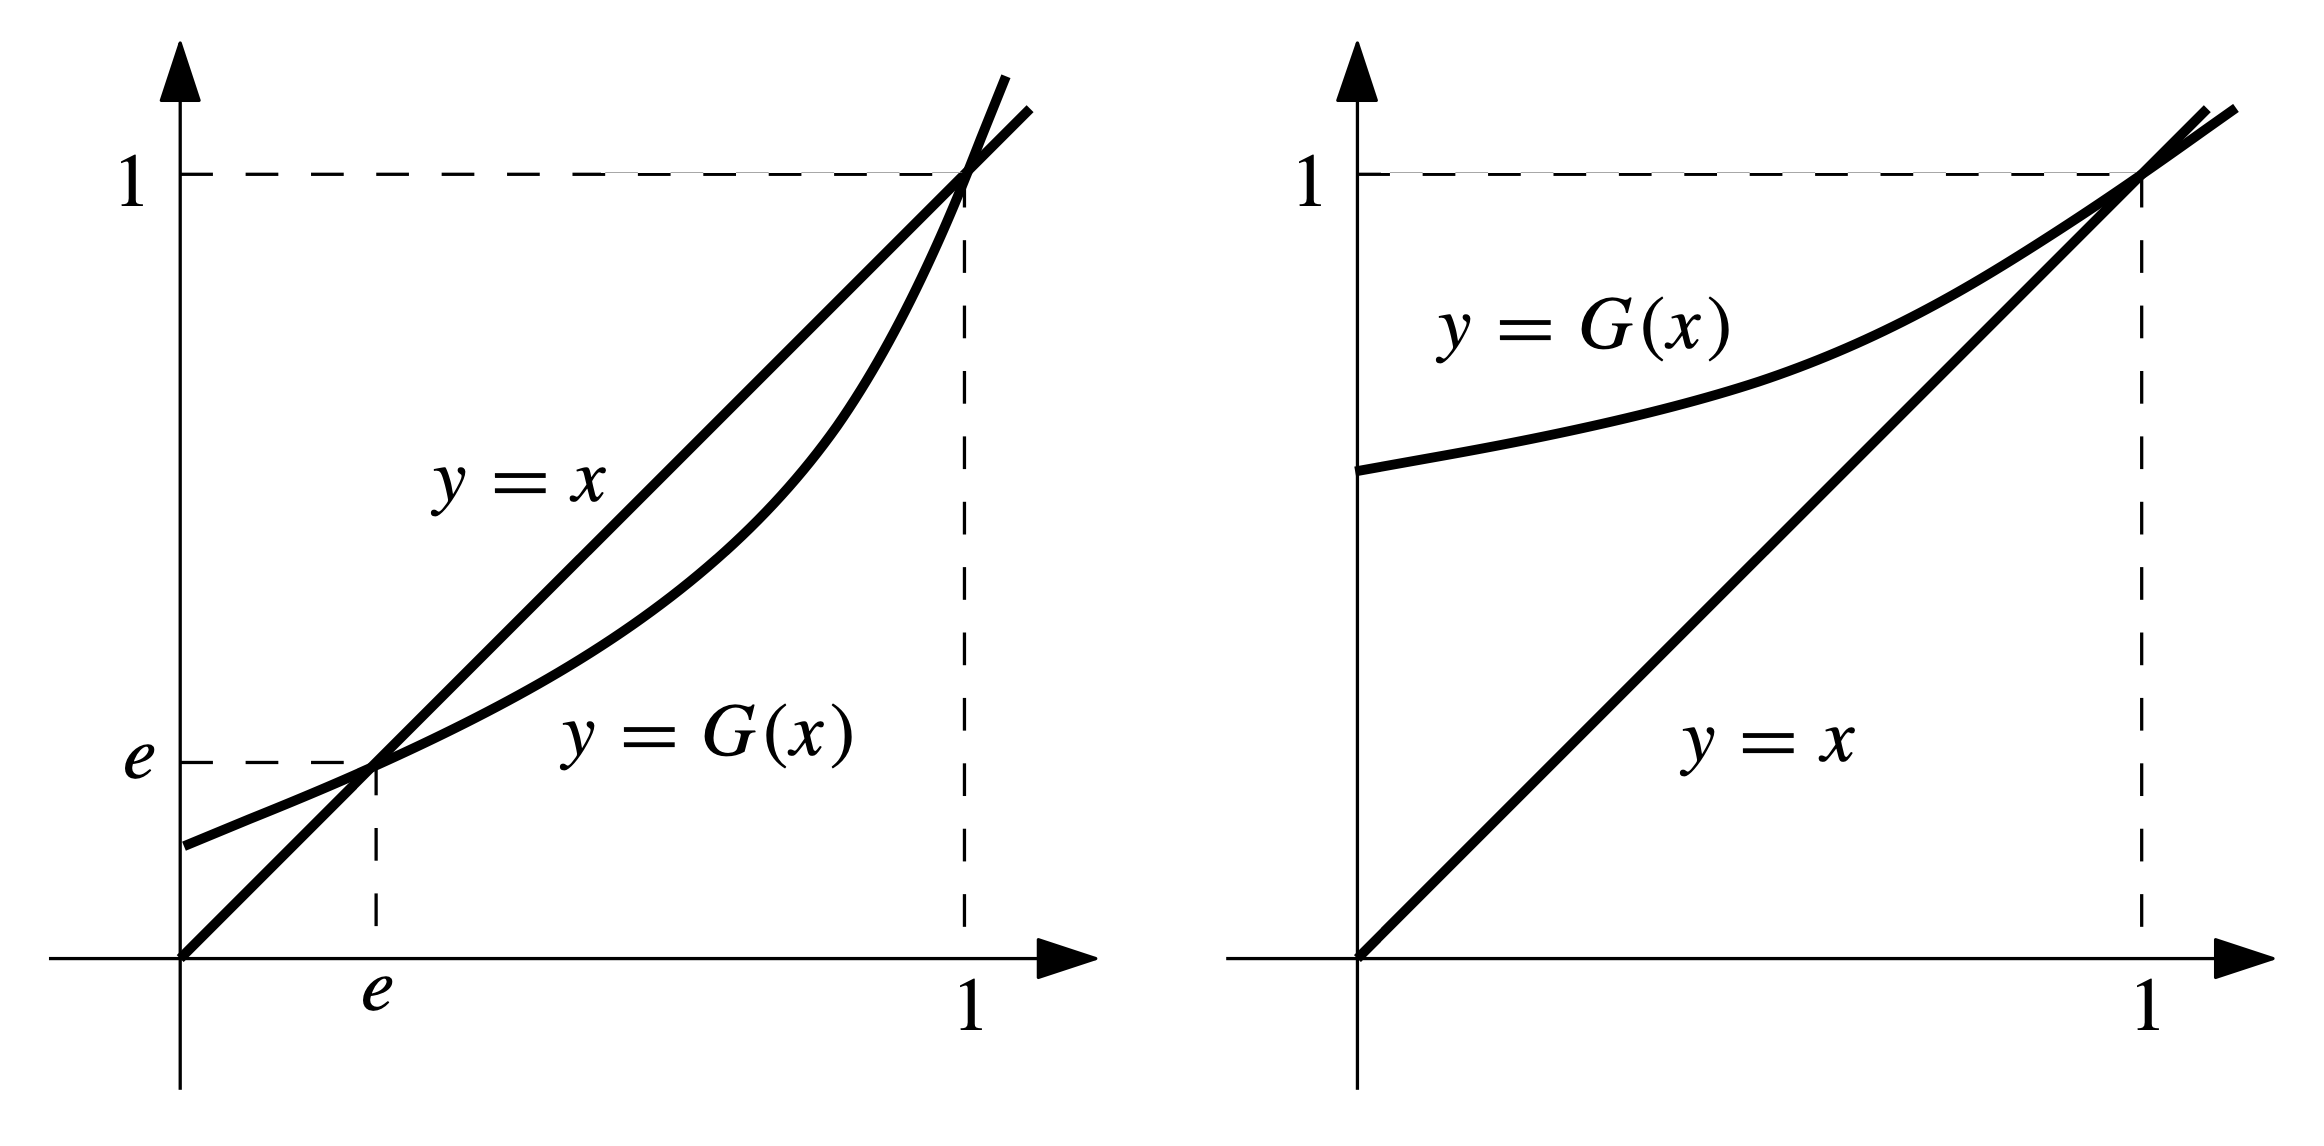
\includegraphics[scale = 0.38]{extinction}

Thus, $\mu \leq 1$ iff $e=1$, i.e., the branching process ultimately goes extinct. (If we want to prove this more rigorously, we might need to show that a concave-up function intersects a linear function with slope 1 at most twice, with the first intersection having $G^{' }(x)<1$ and the second having $G^{' }(x)>1$.)



% ------------------------------------------------------------
% MadHat notebook page 3: Poisson Processes
% ------------------------------------------------------------

\newpage
\section{Poisson Processes}

A \textit{counting process} $N(t)$ for $t\geq 0$ is a continuous stochastic process such that

\begin{itemize}

\item $N(t)$ takes in non-negative integers for each $t$;

\item $N(t)$ is non-decreasing;

\item $N(t)$ is right-continuous, i.e., $N(t)- N(s)$ represents the increment of $N(t)$ in the interval $(s,t]$.

\end{itemize}

A \textit{Poisson process with arrival rate} $\lambda$ is the particular counting process that “follows” the Poisson distribution:

\begin{itemize}

\item $N(0)=0$;

\item $(s_{1},t_{1}]\cap (s_{2},t_{2}]= \emptyset$, then $N(t_{1})- N(s_{1})$ and $N(t_{2})- N(s_{2})$ are independent random variables. (independent increments)

\item The number of events in any interval of length $t$ follows Poisson$(\lambda t)$. (stationary increments dependent solely on $t$)

\end{itemize}

Condition 2 and 3 is explicitly
\[
P(N(t+h)- N(t)=k)=e^{-\lambda h}\frac{(\lambda h)^{k}}{k!}
\]
for arbitrary $t,h,$ and $k\geq 0$.

Similar to what we have done in the theory of Markov chains, different characterizations of stochastic processes may lead to interesting interpretations and properties. As we will soon find out, Poisson processes establish the bridge between the discrete Poisson distribution and the continuous exponential distribution, whose p.m.f. and p.d.f. typically lacked intuition when they were first introduced in a probability class. (As a matter of fact, the exponential distribution is the only continuous distribution with the \textit{lack-of-memory} property, and thus serves as the basis for continuous-time stochastic processes with independent increments.)

Regarding the 2nd and 3rd condition, we have the equivalent infinitesimal definition that, for any $t\geq 0$, $N(t)$ follows the equation that for very small positive $h$, \[P(N(t+h)- N(t)=1)=\lambda h+o(h) \quad \text{and} \quad  P(N(t+h)- N(t)=0)=1- \lambda h+o(h).\]
To illustrate why the two definitions are the same, recall how the Poisson distribution may be interpreted as infinite coin flips. Thus, the coin with success probability $\lambda h$ to increase $N$ by 1 in all intervals with very small length $h$ is what approximates the Poisson process. Note that when $h\rightarrow 0$, the $o(h)$ in the two expressions above will vanish. The rigorous proof of the equivalence between the two definitions requires differential equations and is omitted here.

Both theorems below are easily proven following the infinitesimal definition. 

The superposition of two Poisson processes $N_{1}(t)$ and $N_{2}(t)$ with rate $\lambda _{1}$ and $\lambda _{2}$ by letting $N(t)=N_{1}(t)+N_{2}(t)$ is a new Poisson process with rate $\lambda _{1}+\lambda _{2}$. If events in a Poisson process with rate $\lambda $ has an independent probability $p$ of being type 1, then the counting process of type 1 is a Poisson process with rate $\lambda p$, and the counting process of the remaining events is an \emph{independent} Poisson with rate $\lambda (1- p)$.

Equally important is the characterization using arrival and interarrival times. We define the $n$-th arrival time $S_{n}$ as $\inf \{t\geq 0 : N(t)=n\}$.

It turns out that interarrival times $T_{1}\coloneqq S_{1}- S_{0},T_{2}\coloneqq S_{2}- S_{1},\dots $ between two adjacent events in a Poisson process are all independent and follow Exponential$(\lambda)$. To show this, first we have
\[
P(T_{1}>t)=P(N(t)=0)=e^{- \lambda t},
\]
which tells us that $T_{1}\sim \operatorname{Exponential}(\lambda)$. We can proceed to conclude about $T_{2},T_{3},\dots $ by induction, following
\[
P(T_{n+1}>t \where T_{n}=t_{n},\dots ,T_{1}=t_{1})=P(\text{0 arrival in } (s_{n},s_{n}+t])=e^{- \lambda t},
\]
since the interval $(s_{n},s_{n}+t]$ is of length $t$. (Here $n\geq 1$ and $s_{n}=t_{1}+t_{2}+\dots +t_{n}$, given arbitrary $t_{i}$’s.)

In general, we can show that the Poisson process is a continuous-time Markov chain, and conditioning on any stopping time $T<\infty $ (e.g. the $n$-th arrival time $S_{n}=\sum_{i=1}^{n}T_{i}$ above), $N(T+t)- N(T)$ is a new Poisson process with the same rate $\lambda$, independent of $N$ prior to time $T$. The interarrival result above also follows “directly” from this strong Markov property because all $t_{i}$’s are arbitrary, as we have mentioned above.

It is now clear that $E(S_{n})=\sum_{i=1}^{n}E(T_{i})=n/\lambda $. Furthermore, since $S_{n}$ is the sum of $n$ i.i.d.\ Exponential$(\lambda)$ random variables, it follows the \textit{Gamma distribution} with density
\[
f_{S_{n}}(t)=\lambda e^{- \lambda t}\frac{(\lambda t)^{n- 1}}{(n-1)!}.
\]
We may get this expression above by differentiating both sides of
\[
P(S_{n}>t)=P(N(t)<n)=\sum_{j=0}^{n- 1}e^{- \lambda t}\frac{(\lambda t)^{j}}{j!}.
\]
The last result we discuss here is the relationship between the uniform distribution and the Poisson process. As it turns out, conditioning on the event $N(t)=n$, we have that the $n$ arrival times $S_{1},S_{2},\dots ,S_{n}$ in the interval $[0,t]$ are distributed as the order statistics of $n$ independent Uniform$([0,t])$ random variables.

We briefly sketch why this is true. The key to this is that
\begin{align*}
f(s_{1},s_{2},\dots s_{n} \where N (t)=n) & =\frac{f(s_{1},s_{2},\dots s_{n},n)}{P(N(t)=n)} \\ & = \frac{f(s_{1})f(s_{2}- s_{1})\dots f(s_{n}- s_{n-1})P(s_{n+1}>t)}{P(N(t)=n)} \\
& =\frac{\lambda e^{- \lambda s_{1}}\lambda e^{- \lambda (s_{2}- s_{1})}\dots \lambda e^{- \lambda (s_{n}- s_{n- 1})}e^{- \lambda (t- s_{n})}}{e^{- \lambda t}(\lambda t)^{n}/n!}
=\frac{n!}{t^{n}},
\end{align*}
the exact joint density of the order statistics corresponding to $n$ independent 
Uniform$([0,t])$ random variables.


\end{document}
